\chapter{异构系统协同行为的正确性验证}
\label{ch3}
在本章节,我们首先用SysML建模语言对整个异构系统的架构进行建模,其中用SysML的BDD图来建模系统的组件,用SysML的IBD图来建模系统中各个组件之间的关联关系。由于SysML只是用来建模系统的架构,该建模语言得到的模型不可执行。因此,我们基于FMI标准,将SysML的BDD描述的组件用FMU进行实现,将SysML的IBD图转化为FMU之间的接口配置文件。因此,我们只需要设计协同仿真主算法就可以完成异构系统基于FMI的协同仿真。然而,在我们将基于FMI的可仿真模型输入到协同仿真引擎之中进行仿真之前,我们需要确保该模型的协同行为的正确性,即要保证该模型可以正确的进行协同仿真。为了解决这个问题,我们需要进行两个方面的验证:(1)我们要验证协同仿真主算法的正确性,即算法没有出现死锁以及其他一些特性;(2)我们要验证系统之间各个组件之间关联顺序及数据交互的正确性,其中最主要的要保证多个FMU没有出现环路依赖。在接下来的内容中,我们重点描述如何基于时间自动机理论来验证整个可仿真模型的协同行为的正确性。在第一小节,我们给出整个验证过程的技术框架;第二小节介绍如何对上述的第一个方面进行验证,即协同仿真的主算法的验证;在第三小节中,我们使用一个具体的案例来描述如何对上述的第二个方面进行验证,即异构系统协同行为的验证。
\section{技术框架}
\begin{figure}[htbp]
	\centering
	{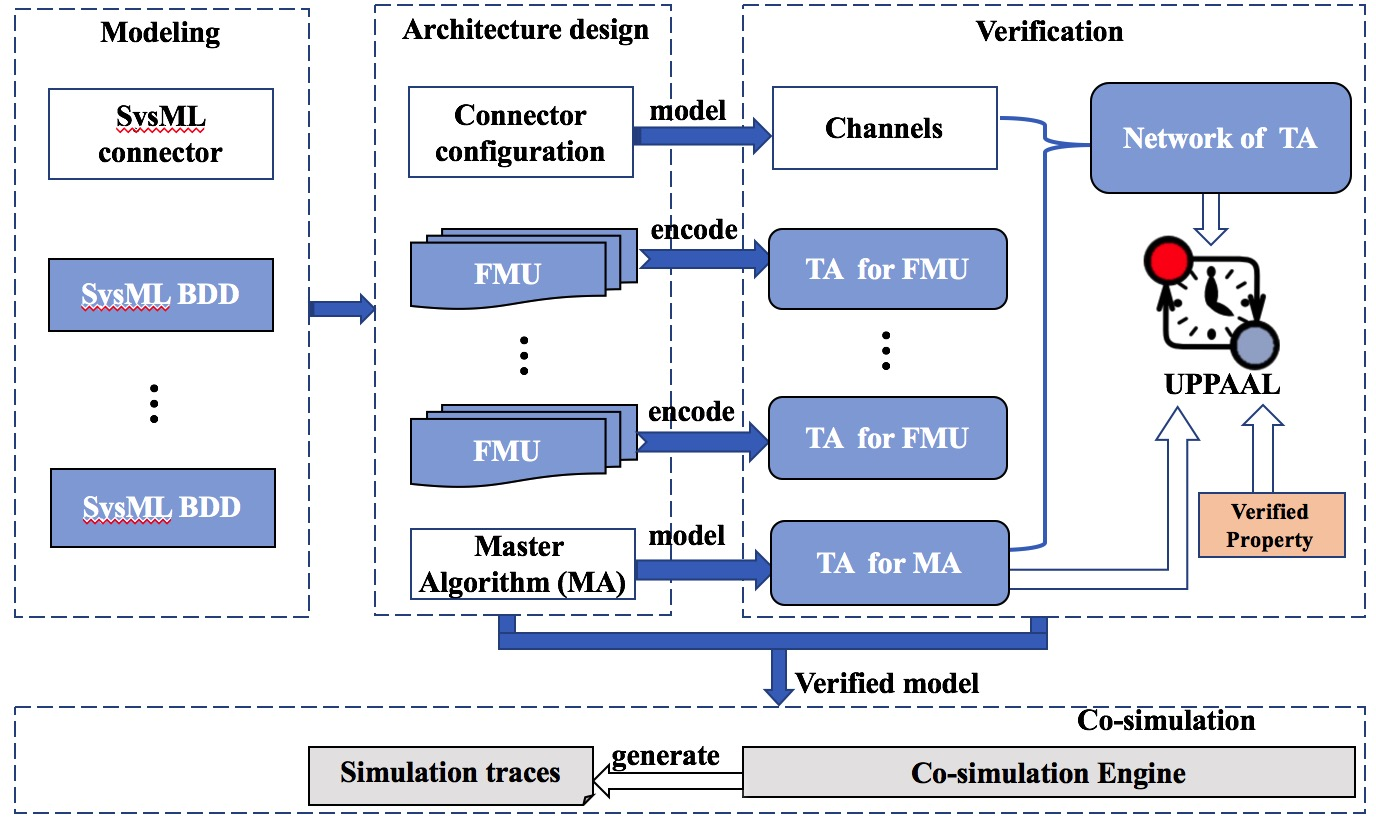
\includegraphics[width=6.0in]{fig/3/framework-3.jpg}}
	%\vspace{0.10in}
	\caption{协同行为正确性验证技术框架图}\label{fra-3}
\end{figure}
图\ref{fra-3}为异构系统协同行为正确性验证的技术框架图. 首先,我们在建模(Modeling)阶段使用SysML的BDD和IBD图来建模整个异构系统的架构。SysML的BDD中的块建模了异构系统的一个个组件;SysML的IBD图描述了各个块之间的连接关系。为了借助协同仿真技术对整个系统进行协同仿真,我们在架构设计(Architecture design)阶段将一个个块用FMU进行实现,同时将IBD图描述的关联关系转化为一个FMU之间的配置文件(Connector configuration)。接下来,我们自己设计了协同仿真的主算法(Master Algorithm,MA)来实现各个FMU之间的交互,同时来驱动协同仿真过程的执行。接下来是协同行为的验证(verification)阶段,也是我们本文的主要贡献点之一。为了验证协同行为的正确性,(1)我们先验证了协同仿真主算法的正确性:首先,我们用时间自动机对协同仿真的主算法进行形式化建模,然后将该时间自动机模型输入到UPPAAL模型检测工具中进行验证 (2)我们验证了整个系统协同行为的正确性:我们提出了一种从FMU到时间自动机的映射规则,我们根据此规则将FMU映射为时间自动机,接下来将FMU之间的配置文件转化为时间自动机的通道(Channels)。这样,我们就得到了一个时间自动机网络(Network of
TA):包括FMU映射成的时间自动机、主算法的时间自动机及各个时间自动机之间的通道)。最后我们将该时间自动机网络和要验证的属性(死锁、可达性、活性等)输入到UPPAAL中来验证该模型是否满足某些属性。一旦验证了协同行为的正确性,我们就可以将通过验证的模型输入到协同仿真的引擎之中进行协同仿真并得到协同仿真的迹。接下来,我们将详细介绍整个协同行为的验证过程。
\section{协同仿真主算法的验证}
在本小节我们首先介绍了三种协同仿真的主算法:固定步长算法、可回滚算法及可预测步长算法,之后我们用时间自动机形式化建模了这几种算法,最后将这几种算法的形式化模型输入到UPPAAL工具中,分别验证了这几种算法的有无死锁、可达性和活性的属性。
\subsection{协同仿真主算法介绍}
协同仿真的主算法用了调度和协同异构系统的多个	FMU组件的执行。每一个FMU都可以被看做一个可独自仿真的黑盒,但是多个FMU之间在某些特定的时刻需要进行数据交互和同步。图\ref{ad-fixedstep}描述了当前三种主要的协同仿真主算法的活动图。在接下来的内容中,我们对这三种算法进行简单的介绍。
\begin{figure}[htbp]
\centering{
		\subfigure[固定步长算法]{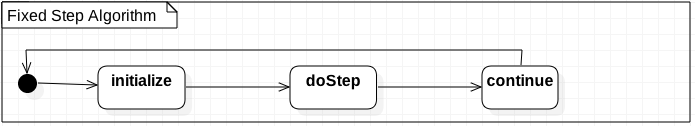
\includegraphics[width=4.5in,height=0.8in]{fig/3/MA1.png}
			\label{sd_fixedstep}}
		\hfil
		\subfigure[可回滚算法]{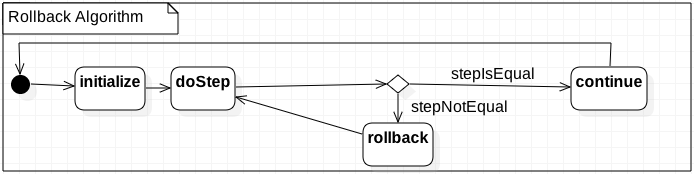
\includegraphics[width=4.5in,height=0.9in]{fig/3/MA2.png}
			\label{sd-rollback}}	
		\subfigure[可预测步长算法]{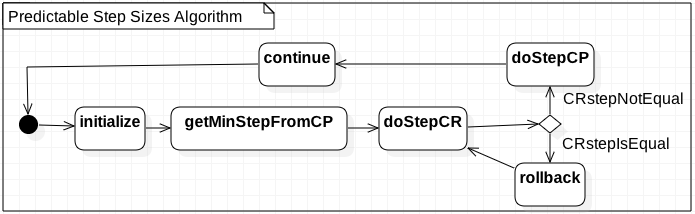
\includegraphics[width=4.5in,height=1.1in]{fig/3/MA3.png}
			\label{sd-pre}}		
	\caption{三种协同仿真主算法的活动图}
	\label{ad-fixedstep}
	}
\end{figure}
\subsubsection{固定步长算法}
对于固定步长算法\cite{BromanBGLMTW13},所有的FMU都有一个相同的步长。当协同仿真主算法在$t$时刻调用$doStep$函数执行步长$h$时,所有的FMU将从$t$时刻执行$h$步长并到达$t+h$时刻。在执行下一个$doStep$函数之前,要确保所有的FMU都执行完了上一个步长并且完成了数据交换。固定步长算法的活动图如图\ref{sd_fixedstep}所示,该活动图主要包含三个活动: $initialize$, $doStep$ 和 $continue$,首先对所有的FMU进行初始化,之后调用$deStep$函数进行仿真,最后在$continue$活动中完成FMU的数据交换。 在固定步长算法中,只要保证每个FMU的仿真是可靠的,则可以保证整个仿真过程的可靠性。但是,如果在某个FMU的仿真过程中出现错误,则会导致整个协同仿真过程出错。为了克服固定步长算法的缺陷,出现了可回滚的算法。
\subsubsection{可回滚算法}
FMI2.0相对于FMI1.0添加了几个重要的特性,它支持了对于FMU状态的保存和回滚。例如,主算法调用$FMU_{1}$和$FMU_{2}$的$doStep$函数执行$h$步长,但是$FMU_{1}$接受了该步长且$FMU_{2}$拒绝了该步长,则$FMU_{1}$和$FMU_{2}$都会执行$h$步长然后回滚到上一个时间点。可回滚算法的活动图如图\ref{sd-rollback}所示,相比固定步长算法,可回滚算法要求所有的FMU支持$rollback$方法, 且当某个FMU拒绝该步长时,所有的FMU将会回滚到上一个步长执行完之后的时间点。
\subsubsection{可预测步长算法}
如果可以预测FMU下一步能执行的最大步长(FMU在不错过事件时,能执行的仿真的最长时间),则可以大大提高协同仿真的效率。因此,论文\cite{BromanBGLMTW13}提出了$GetMaxStepSize$函数来预测FMU下一步能执行的最大步长,有了该函数的支持,就出现了可预测步长算法。图\ref{sd-pre}为可预测步长算法的活动图,首先,所有的FMU进行初始化,然后支持$GetMaxStepSize$函数的FMU在$getMinStepFromCP$活动中预测他们下一步能执行的最大步长,并且在所有的最大步长中选择最小的一个$h$作为所有FMU下一步执行的步长,之后所有的FMU执行$h$步长,如果所有的FMU都接受了该步长,则所有的FMU仿真该步长然后进行下一步。如果有FMU拒绝了该步长,则将所有的FMU回滚到上一个时间点,然后选择一个更小的步长进行仿真。
\subsection{协同仿真主算法的建模和验证} 
我们用时间自动机将三种不同类型的主算法进行形式化建模,图\ref{ta-master}是三种主算法的时间自动机模型。固定步长算法的时间自动机模型包含$Init$和$doStep$两个状态,且与$FMU$通过$continue$信道进行通信。 可回滚算法包括$Init$、$DoStep$和$Continue$三个状态。如果所有的FMU都接受了下一步要进行仿真的步长,则可回滚算法对应的时间自动机将发送$continue$信号,且迁移到$Continue$状态;否则,将发送$rollback$信号,且返回到上一个状态。可预测步长算法包括$Init$, $find \_ CP \_ MIN$, $DoStep$, $writeCP$四个状态。首先他们获得支持预测步长算法的多个FMU的最大步长,然后取所有最大步长的最小值$step1$ 。然后执行该步长,如果所有的FMU都接受则发送$continue$信号并迁移到下一个状态,否则发送$rollback$信号并回滚到$DoStep$ 状态。
\begin{figure}[htbp]
\centering{
		\subfigure[固定步长算法的时间自动机模型]{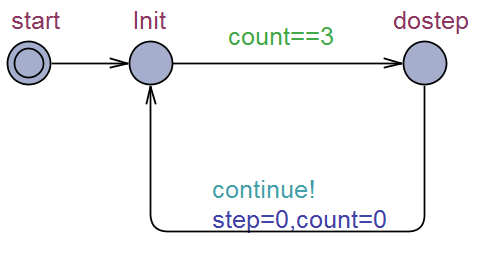
\includegraphics[width=2.0in,height=1.2in]{fig/3/fixedstep_master.png}
			\label{ta_fixedstep}}
		\hfil
		\subfigure[可回滚算法的时间自动机模型]{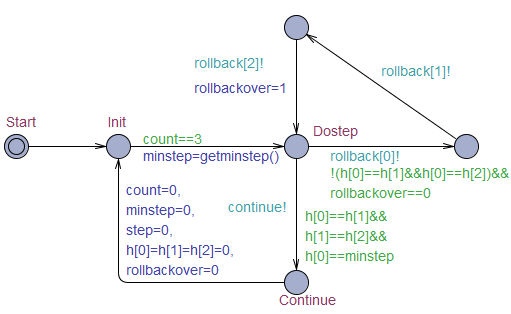
\includegraphics[width=3.0in,height=1.6in]{fig/3/rollback_master.png}
			\label{ta-rollback}}	
		\subfigure[可预测步长算法的时间自动机模型]{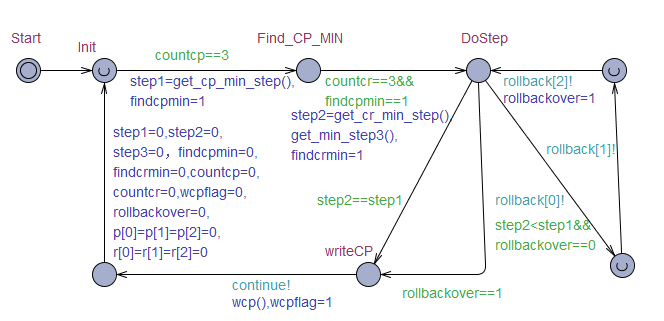
\includegraphics[width=5.0in,height=2.0in]{fig/3/pma_master.png}
			\label{ta-pre}}		
	\caption{三种不同主算法的时间自动机模型。}
	\label{ta-master}
	}
\end{figure}

UPPAAL是基于时间自动机理论对实时系统进行验证的工具,其中使用到的时间自动机模型增加了整型变量、多种数据类型及同步信号等扩展。我们使用UPPAAL工具验证了这三个模型的可达性、活性及死锁。具体的验证属性如下所示:
\begin{itemize}
\item
$E \langle\rangle master.dostep$, $E\langle\rangle master.Continue$ and $E\langle\rangle master.writeCP$是可达性验证,用来验证这些系统状态是否可达;
\item
$master.Init -> master.dostep$, $master.Init -> master.Continue$ and $master.Init -> master.Continue$是活性验证。如果主算法可以到达前一个状态,那么它最终也会到达后一个状态。
\item
$A[] not deadlock$ 是死锁的验证, 用来验证主算法是否存在死锁。
\end{itemize}
实验的结果如表\ref{ta_r}所示,从表中我们可以看出不存在死锁,且可达性和活性都满足,说明我们的主算法是正确的。例如:属性$A[]~not~deadlock$满足,说明主算法不存在死锁; 属性$E\langle\rangle~master.doStep$ 满足,说明系统最终会到达$doStep$状态。 总结来说,我们在这一小节验证了我们所用到的协同仿真的主算法的正确性。
\begin{table}
\caption{主算法的验证实验结果}
\centering
\begin{tabular}{c c c}
          \hline
          主算法 & 验证属性 & 结果\\
       \hline
        \multirow{2}{2.0cm}{固定步长}
                & $A[]~not~deadlock$ & True\\
                & $master.Init -> master.dostep$ & True\\
                & $E\langle\rangle~master.dostep$ & True\\

        \hline
        \multirow{2}{2.0cm}{可回滚}
                & $A[]~not~deadlock$ & True\\
                & $master.Init -> master.Continue$ & True\\
                & $E\langle\rangle~master.Continue$ & True\\

        \hline
        \multirow{2}{2.0cm}{可预测}
                & $A[]~not~deadlock$ & True\\
                & $master.Init -> master.writeCP$ & True\\
                & $E\langle\rangle~master.writeCP$ & True\\
        \hline
\end{tabular}
\label{ta_r}
\end{table}

\section{异构系统协同行为的验证}
在本小节,我们使用一个水箱的案例对整个协同行为的验证过程进行详细的描述。由于,在验证过程中,需要用时间自动机对FMU进行形式化描述,我们首先给出了从FMU到时间自动机的映射规则,然后我们使用SysML对整个系统进行架构设计,之后基于FMI标准对系统的各个组件进行实现,并给出多个FMU之间的连接关系配置,最后我们用时间自动机建模了FMU的形式化模型,并输入到UPPAAL工具中针对验证属性进行验证分析。
\subsection{FMU到时间自动机的映射} 
在本文的第二章的预备知识中,我们给出了FMU和时间自动机的语法及语义,下面我们根据第二章的语法语义给出FMU和时间自动机的映射关系。我们发现FMU和时间自动机的语义之间存在一定的关联。FMU的语义关注于FMU的执行序列,也就是状态随着时间的不断迁移;因此,时间自动机的执行迹跟FMU的执行序列十分相似,也是状态随着时间的迁移序列。因此,我们使用时间自动机来对FMU进行形式化描述,从而来分析多个FMU之间的协同行为。
给定一个FMU$F=(S,U,Y,D,s_{0},set,get,doStep)$, 我们可以根据他们执行语义之间的关联,将FMU用时间自动机$\textit{A}=(L,l_{0},E,I)$进行形式化描述:
\begin{itemize}
\item
$L$是时间自动机的有限位置集合。因此,时间自动机语义模型$L_{\textit{A}}$中的状态可以看做为FMU中的状态,即$(l,v) \Rightarrow s$.
\item
时间自动机语义模型$L_{\textit{A}}$中的初始状态可以看做为FMU中的初始状态$F$, 即$(l_{0},v_{0}) \Rightarrow s_{0}$. 
\item
FMU中的输入变量$u \in U$可以看做为时间自动机的$Act_{i} \cup \{absent\}$.
\item
FMU的输出变量$y \in Y$可以看做为时间自动机的$Act_{o} \cup \{absent\}$.
\item
An input action $e \in Act_{i}$ is such that the function $set$ of $F$ sets the input variable $u$ with a given value. 
\item
An output action $e \in Act_{o}$ indicates that the function $get$ of $F$ gets the output variable $y$. The set of values in the $Act_{i}$ can be seen as $Y$ of $F$.  
\item
The communication between the TA is the same as the I/O dependencies information between the FMUs. $(u,y) \in D$ denotes that output $y$ depend on input $u$. The output actions also depend on the input actions in TA.
\item
For any $e \in Act$ of A, there is a transition $s \xrightarrow{e} s^{\prime}$, which may be found after the function $doStep$ executed. For instance, if there is a transition $l \xrightarrow{e} l^{\prime}$ in $A$, at the same time $doStep(s,h)$ may be called which indicates that $F$ accepts the time step $h$ and reaches the new state $s^{\prime}$. However, the time step $h$ may be rejected, if there is a rollback behaviour happens, the transition in TA could be an edge $l^{\prime} \xrightarrow{e} l$, which denotes that a location travels to the former location.

\end{itemize}
\begin{figure}[htbp]
	\centering	{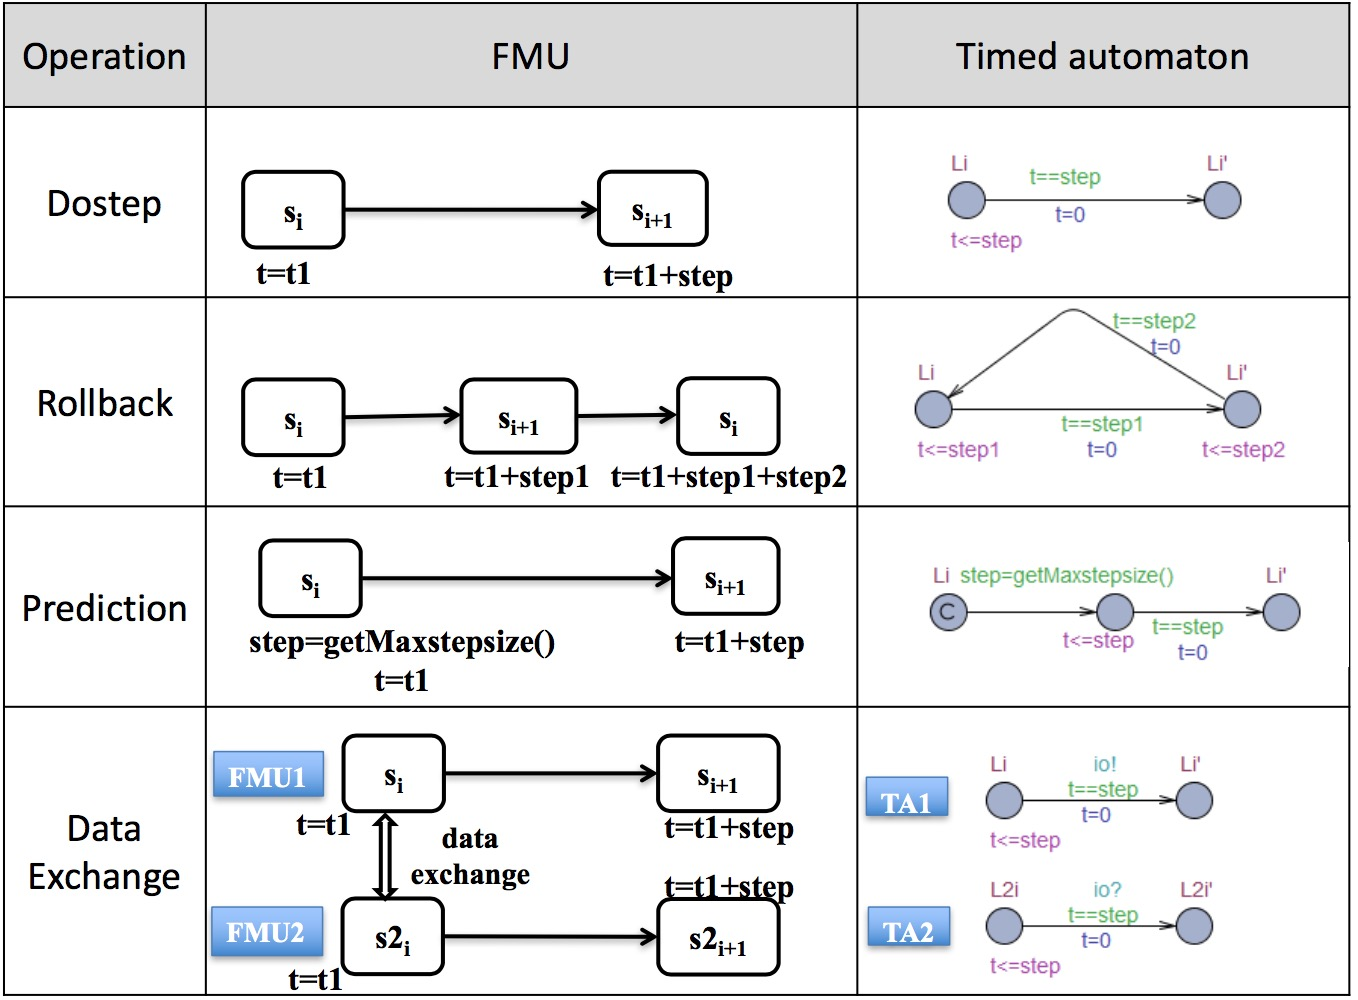
\includegraphics[width=5.0in,height=3.5in]{fig/3/abstractRole.png}}
	\caption{Encoding rules from FMU to TA.}
	\label{fmutota}
\end{figure}

It is not easy to map FMUs to TA directly. S. Tripakis encodes TA as FMUs in \cite{Tripakis15}. Inspired by it, we propose some encoding rules to encode FMUs as TA according to the congruent relationships. As we can see in the Fig.~\ref{fmutota}, given a state $s_{i}$ at $t_{1}$ in FMU, the operation $Dostep$ makes FMU reach a new state $s_{i+1}$ at $t_{1}+step$. This situation can be encoded as a transition in TA, in which a location $L_{i}$ delays $step$ time and goes to a new location $L_{i}^{\prime}$.

For the operation $Rollback$, given a state $s_{i}$ at $t_{1}$ in FMU, the FMU will do a $step1$ to $s_{i+1}$ at $t_{1}+step1$, and then, the operation $rollback$ makes FMU reach the former state $s_{i}$. For this situation, it can be encoded as location $L_{i}$ delays $step1$ time units and reach a new location $L_{i}^{\prime}$ after a transition, and then returns to the former location $L_{i}$. 

For the operation $Prediction$, given a state $s_{i}$, FMU can get max step size for next step, and then reach a new state $s_{i+1}$ at $t_{1}+step$. For TA, it gets max step size in location $L_{i}$, then it delays $step$ time units and reach a new location $L_{i}^{\prime}$ .

For $Data Exchange$ between two FMUs in state $s_{i}$ at $t_{1}$, they exchange data at $t_{1}$ and then do the same step to $s_{i+1}$. In TA, there will be a signal $io$ to make the two FMUs do the same step from $L_{i}$ to $L_{i+1}$ after data exchange.

To bridge the semantic gaps between FMU and TA, we provide proper encoding rules to formalize FMUs as TA. It lays the foundation to analyse coordination of CPS with TA-based model checking. 
%Limited to the length of this paper, we don't prove the correctness of encoding rules. But the encoding process is semantic-preserve. In section \ref{sec:sysml}, we apply these encoding rules to the water tank case study. According to the simulation results, we can find that the encoding rules work well.
As for the correctness of encoding rules, we analyse the equivalence of execution fragments as following:
\begin{itemize}
\item
For the encoding rule of $Dostep$ operation, the execution fragments of FMU and TA are ($s_{i}$, $t_{1}$), ($s_{i+1}$, $t_{1}+step$) and ($l_{i}$, $t$), ($l_{i}^{\prime}$, $t+step$). It means that TA and FMU execute $step$ time units, and jump to a new state or location.
\item 
For encoding rule of $Rollback$ operation, the execution fragments of FMU and TA are ($s_{i}$, $t_{1}$), ($s_{i+1}$, $t_{1}+step1$), ($s_{i}$, $t_{1}+step1+step2$) and ($l_{i}$, $t$), ($l_{i}^{\prime}$, $t+step1$), ($l_{i}$, $t+step1+step2$). It means that TA and FMU execute $step1$ time units, and jump to a new state or location, and then execute $step2$ time units, return to the previous state or location. 
\item
For the encoding rule of $Prediction$, the execution fragments of FMU and TA are ($s_{i}$, $t_{1}$), ($s_{i+1}$, $t_{1}+step$) and ($l_{i}$, $t$), ($l_{i}^{\prime}$, $t+step$). It means that TA and FMU predict the step size $step$, and then execute $step$ time units.
\item
For the encoding rule of $Data Exchange$ operation, the execution fragments of FMU1 and TA1 are ($s_{i}$, $t_{1}$), ($s_{i+1}$, $t_{1}+step$) and ($l_{i}$, $t$), ($l_{i}^{\prime}$, $t+step$). The execution fragments of FMU2 and TA2 are ($s2_{i}$, $t_{1}$), ($s2_{i+1}$, $t_{1}+step$) and ($l2_{i}$, $t$), ($l2_{i}^{\prime}$, $t+step$). It means that FMUs or TA exchange data, and then execute $step$ time units.
\end{itemize}
We have analysed the whole execution trace of FMU and TA for these encoding rules. According to the encoding rules, we find that the execution traces of FMUs and TA are equivalent which means the encoding rules work well. In section \ref{sec:sysml}, we apply these encoding rules to the water tank system. According to the simulation fragments of the case study, we also find that the encoding rules work well.
\subsection{基于SysML的架构建模} 
\subsection{基于FMI的连接关系配置} 

\subsection{协同行为的验证分析} 
\section{本章小结}

